\documentclass{article}

\usepackage{xcolor}
\usepackage{hyperref}
\definecolor{COLOR_MEAN}{HTML}{f0f0f0}
\definecolor{LINK_COLOR}{HTML}{636EFA}
\hypersetup{
	colorlinks=true,
	linkcolor=LINK_COLOR,
	urlcolor=LINK_COLOR,
	citecolor=LINK_COLOR,
}

% if you need to pass options to natbib, use, e.g.:
%     \PassOptionsToPackage{numbers, compress}{natbib}
% before loading neurips_2024


% ready for submission
%\usepackage{neurips_2024}


% to compile a preprint version, e.g., for submission to arXiv, add add the
% [preprint] option:
% \usepackage[preprint]{neurips_2024}


% to compile a camera-ready version, add the [final] option, e.g.:
\usepackage[final]{neurips_2024}


% to avoid loading the natbib package, add option nonatbib:
%    \usepackage[nonatbib]{neurips_2024}


\usepackage[utf8]{inputenc} % allow utf-8 input
\usepackage[T1]{fontenc}    % use 8-bit T1 fonts
\usepackage{hyperref}       % hyperlinks
% \usepackage{url}            % simple URL typesetting
\usepackage{xurl}
\usepackage{booktabs}       % professional-quality tables
\usepackage{amsfonts}       % blackboard math symbols
\usepackage{nicefrac}       % compact symbols for 1/2, etc.
\usepackage{microtype}      % microtypography
\usepackage{xcolor}         % colors
\usepackage{tabularx}
\usepackage{booktabs}
\usepackage{amsmath}
\usepackage{listings}
\usepackage{xspace}
\usepackage{cleveref}
\usepackage{multirow}
\usepackage{multicol}
\usepackage{subcaption}

\usepackage{algorithm} 
\usepackage{algpseudocode}
\usepackage{mathrsfs}
\usepackage{tikz}

\usepackage[symbol]{footmisc}
\definecolor{ntured}{HTML}{D71440}
\hypersetup{
    colorlinks=true,     
    urlcolor=ntured,
}



\newcommand{\bplustree}{B+ tree\xspace}


% \title{SC3020 Project 1}


% The \author macro works with any number of authors. There are two commands
% used to separate the names and addresses of multiple authors: \And and \AND.
%
% Using \And between authors leaves it to LaTeX to determine where to break the
% lines. Using \AND forces a line break at that point. So, if LaTeX puts 3 of 4
% authors names on the first line, and the last on the second line, try using
% \AND instead of \And before the third author name.


% \author{
% }

\usepackage{graphicx}

\begin{document}
	
\begin{titlepage}
	\begin{figure}[!t]
		\centering
		
\includegraphics[width = 4.3in]{title/logo.pdf}
	\end{figure}
	
	\centering
	\huge{\textbf{SC3020 Database Systems Principles}}\\[0.2in]
	\huge{\textbf{Project 1 Report}}\\[2in]
        \small {Code: \url{https://bit.ly/SC3020Project1}} \\
        \small {Presentation Video: \url{https://bit.ly/SC3020Project1Video}}
	
	%	\LARGE{\textbf{YOUR NAME}}\\
	%	\normalsize{Matriculation number}\\[0.2in]
	
	\begin{table}[h]
		\centering
		\resizebox{\textwidth}{!}{%
			\begin{tabular}{lll}
				\toprule
				\textbf{Name} & \textbf{Email} & \textbf{Matric Number} \\
				\midrule
                    Cui Nan & C220133@e.ntu.edu.sg & U2221495L\\
				Pu Fanyi & FPU001@e.ntu.edu.sg & U2220175K \\
				Shan Yi & SH0005YI@e.ntu.edu.sg & U2222846C\\
                    Zhang Kaichen & ZHAN0564@e.ntu.edu.sg & U2123722J \\
                    Tian Yidong & YTIAN006@e.ntu.edu.sg & U2220492B \\
				\bottomrule
			\end{tabular}%
		}
	\end{table}

	
	
    
	
	%	\large{A Final Year Report submitted to Asian School of the Environment, Nanyang Technological University in partial fulfilment of the requirements for the Degree of }\\[0.1in]
	
	\vspace{0.5in}
    \LARGE{College of Computing and Data Science}\\
	\LARGE{Nanyang Technological University, Singapore}\\[0.3in]
	
	
	\LARGE{2024/2025 Semester 1}
	\newpage
\end{titlepage}
	
% \maketitle

% \begin{abstract}
%     lalala
% \end{abstract}


\section{Introduction}
\label{sec:intro}

This project focuses on the design and implementation of two key components of a database management system: storage and indexing.

Our report is structured as follows:

\begin{enumerate}
    \item First, we illustrate the design of our storage component, where data is stored in blocks on computer disks.
    \item Next, we describe the implementation of our \bplustree and the process of storing the index on the disk.
    \item Finally, we present the statistics and experimental results obtained using our database system.
\end{enumerate}


\section{Storage Components}
\label{sec:storage}

In this section, we illustrate the design of our storage components. We begin by listing all the components in our design, followed by a demonstration of how each component interacts with the others.

\subsection{Data Components}
\label{subsec:data-components}

The data components primarily consist of the following objects:

\begin{itemize}
    \item \textbf{BlockData}: This object stores the actual data. The data is stored as an array of bytes, with the size determined by the block size of different computers.
    \item \textbf{BlockPtr}: This object points to the position of the \texttt{BlockData}. Given a file stream, the \texttt{BlockPtr} can access a specific range of positions within that file stream.
    \item \textbf{DataPtr}: This object points to a specific range of positions within a \texttt{BlockData}. In real-time operations, a \texttt{BlockPtr} is used to manage the loading and storing of the \texttt{DataPtr}.
    \item \textbf{Record}: A \texttt{Record} is a subclass of the \texttt{DataPtr}. It can access a specific range within the \texttt{BlockPtr}, corresponding to the size of the record.
    \item \textbf{Schema}: The \texttt{Schema} manages the field names and data types of a table. A Schema object is used to determine the number of bytes required to write input data and the number of bytes needed to read a record when loading from an array of bytes.
\end{itemize}

During the reading and writing processes, all data is converted into a uniform format, specifically an array of bytes. For example, an int or float data type is converted into an array of size 4 bytes, while a bool data type is converted into an array of size 1 byte. During reading, we access only the \texttt{BlockPtr} or \texttt{RecordPtr}, which points to a specific location in the data. When a specific range is needed, the corresponding byte array is loaded into memory. A detailed illustration of our storage format and components is provided in ~\Cref{fig:storage-component}.

\begin{figure}[t]
    \centering
    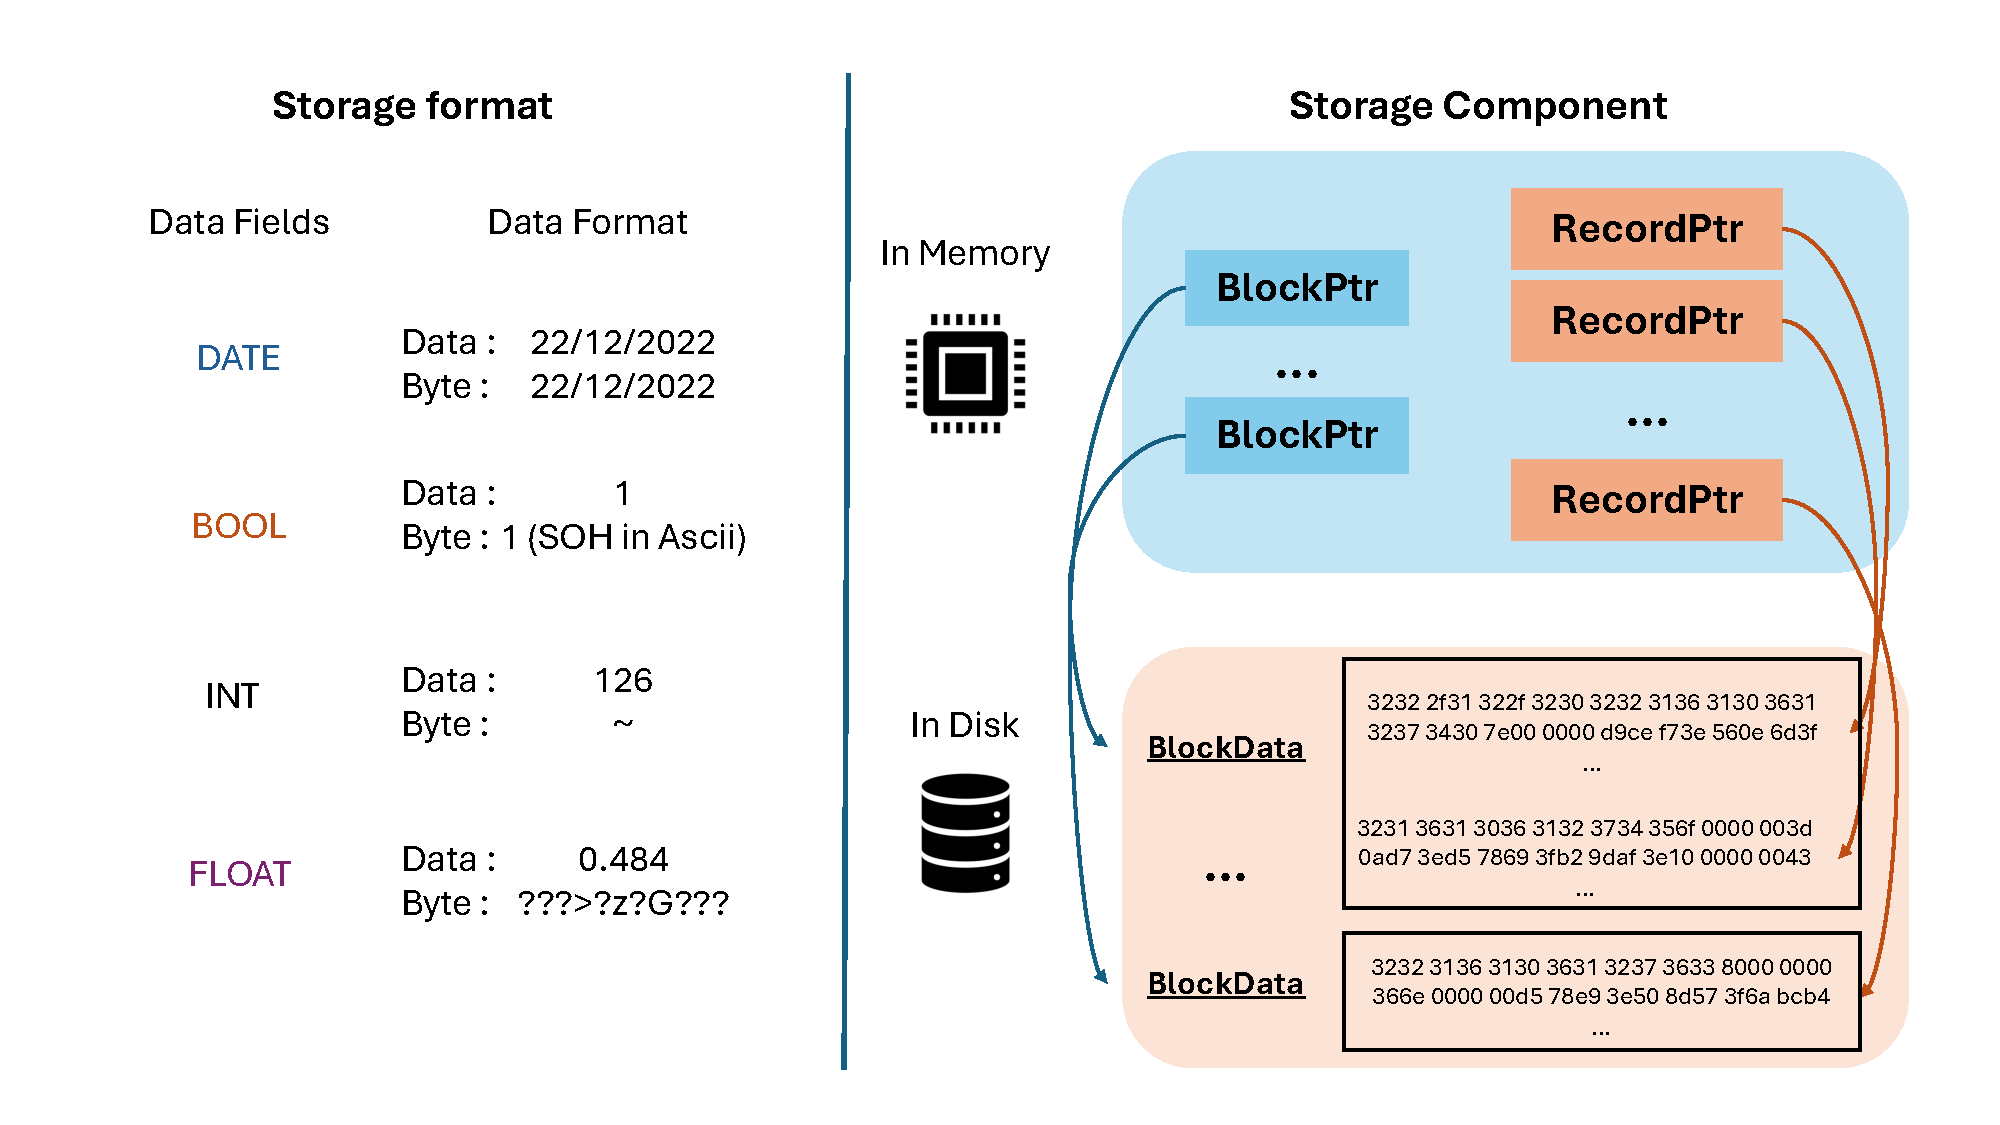
\includegraphics[width=1\linewidth]{figures/Storage_component.pdf}
    \caption{Illustration of the storage components design in our project. All the data are converted into array of Byte and store in the disk. Only pointers that points to the offset position will be stored in memory.}
    \label{fig:storage-component}
\end{figure}


\subsection{Controller Components}
\label{subsec:controller}

\begin{figure}[t]
    \centering
    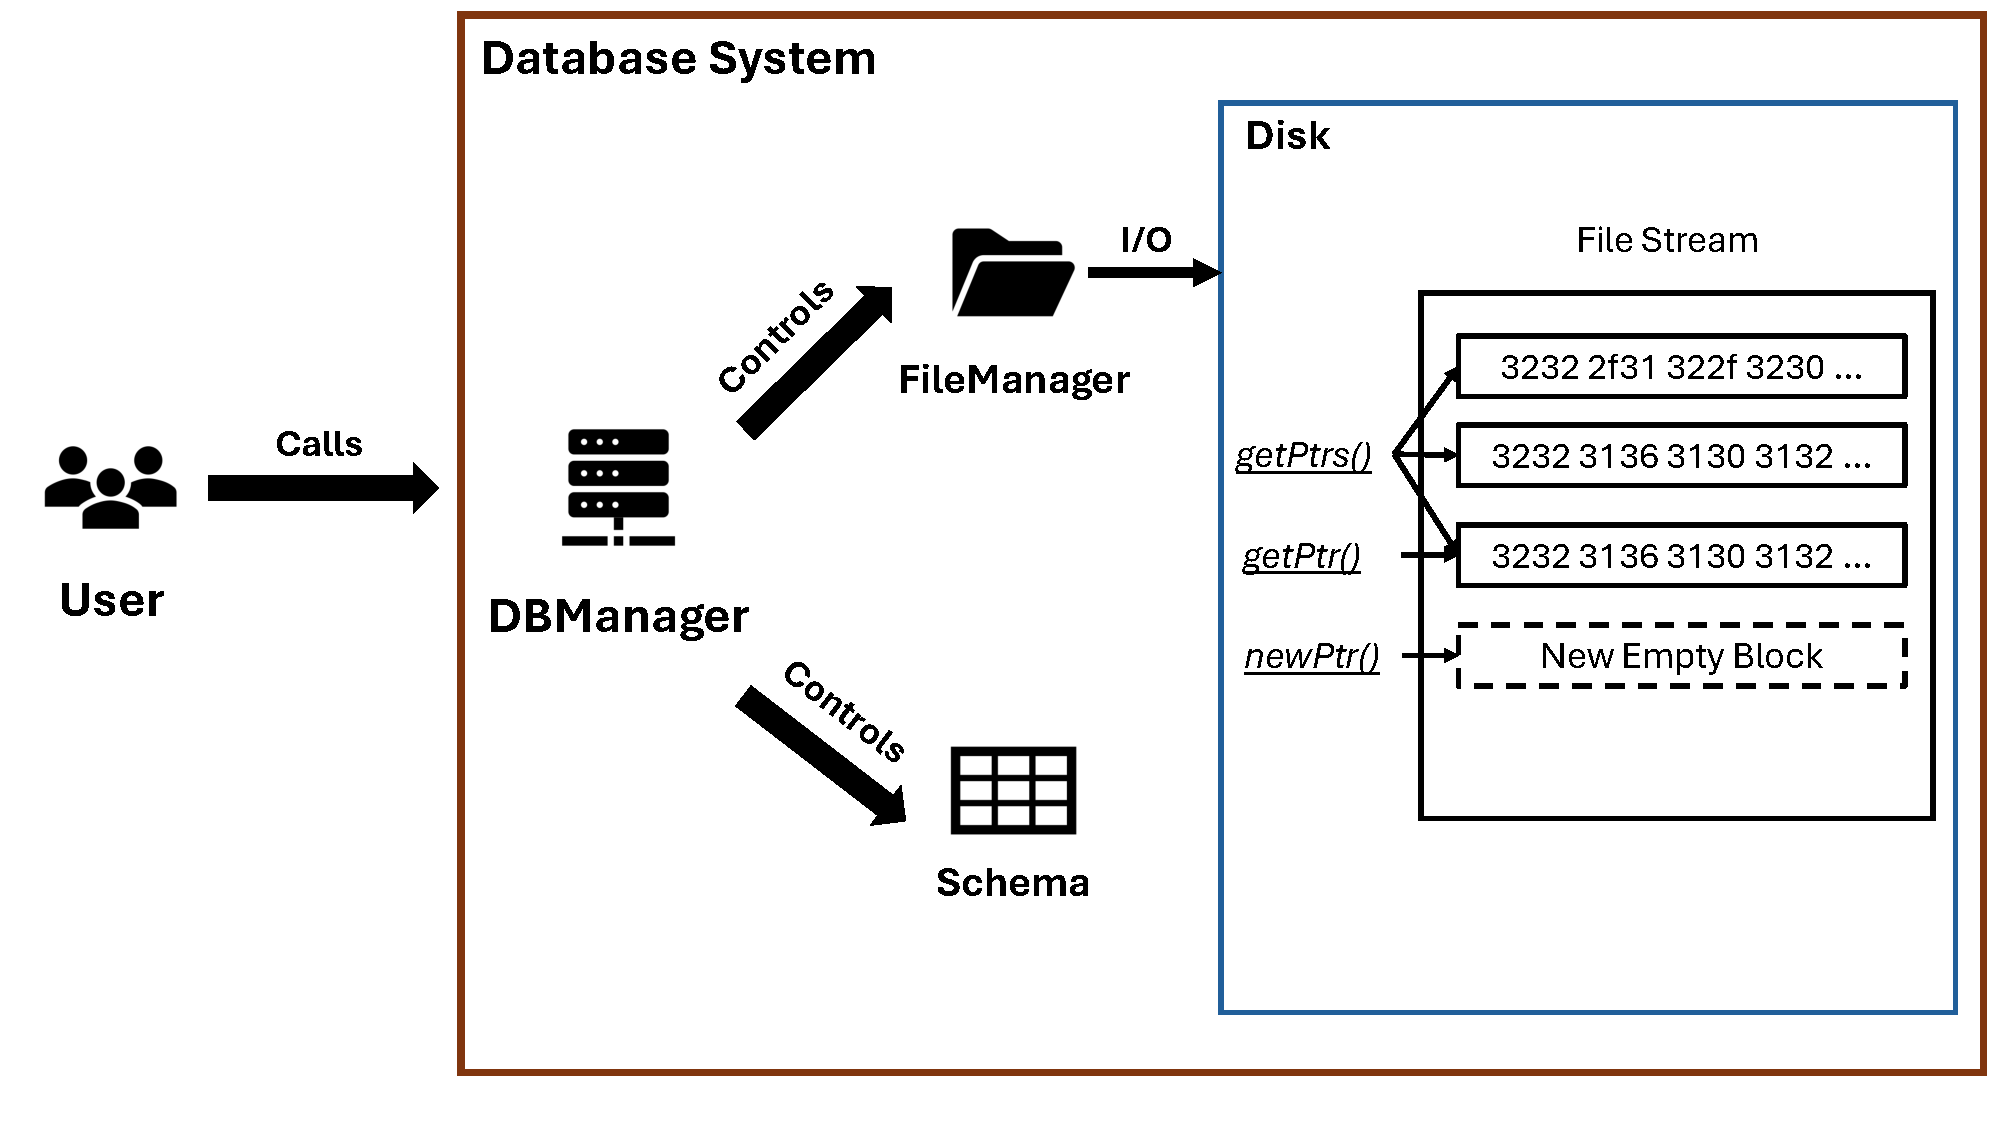
\includegraphics[width=1\linewidth]{figures/Cotroller.pdf}
    \caption{The controller components in how user interactive with the database.}
    \label{fig:Controller}
\end{figure}

We will now illustrate our controller components, which are primarily responsible for managing the data components described in ~\Cref{subsec:data-components}. The two main controller objects are as follows:

\begin{itemize}
    \item \textbf{FileManager}: This object manages all BlockPtr instances and the file stream. It handles read and write operations between the file and the buffer pool.
    \item \textbf{DataBaseManager}: This object controls the database, using the FileManager to load data or allocate new memory blocks for data storage. It also oversees the process of reading from the original text file or from the byte array, returning a pointer to the record position.
\end{itemize}

When interacting with the user, the DataBaseManager calls the FileManager to allocate new memory or read from existing memory. During a \texttt{load()} operation, the DataBaseManager initiates an I/O operation for one block, as detailed in ~\Cref{fig:Controller}.

\subsection{Buffer Pool}
\label{subsec:io-control}

\begin{figure}[ht]
    \centering
    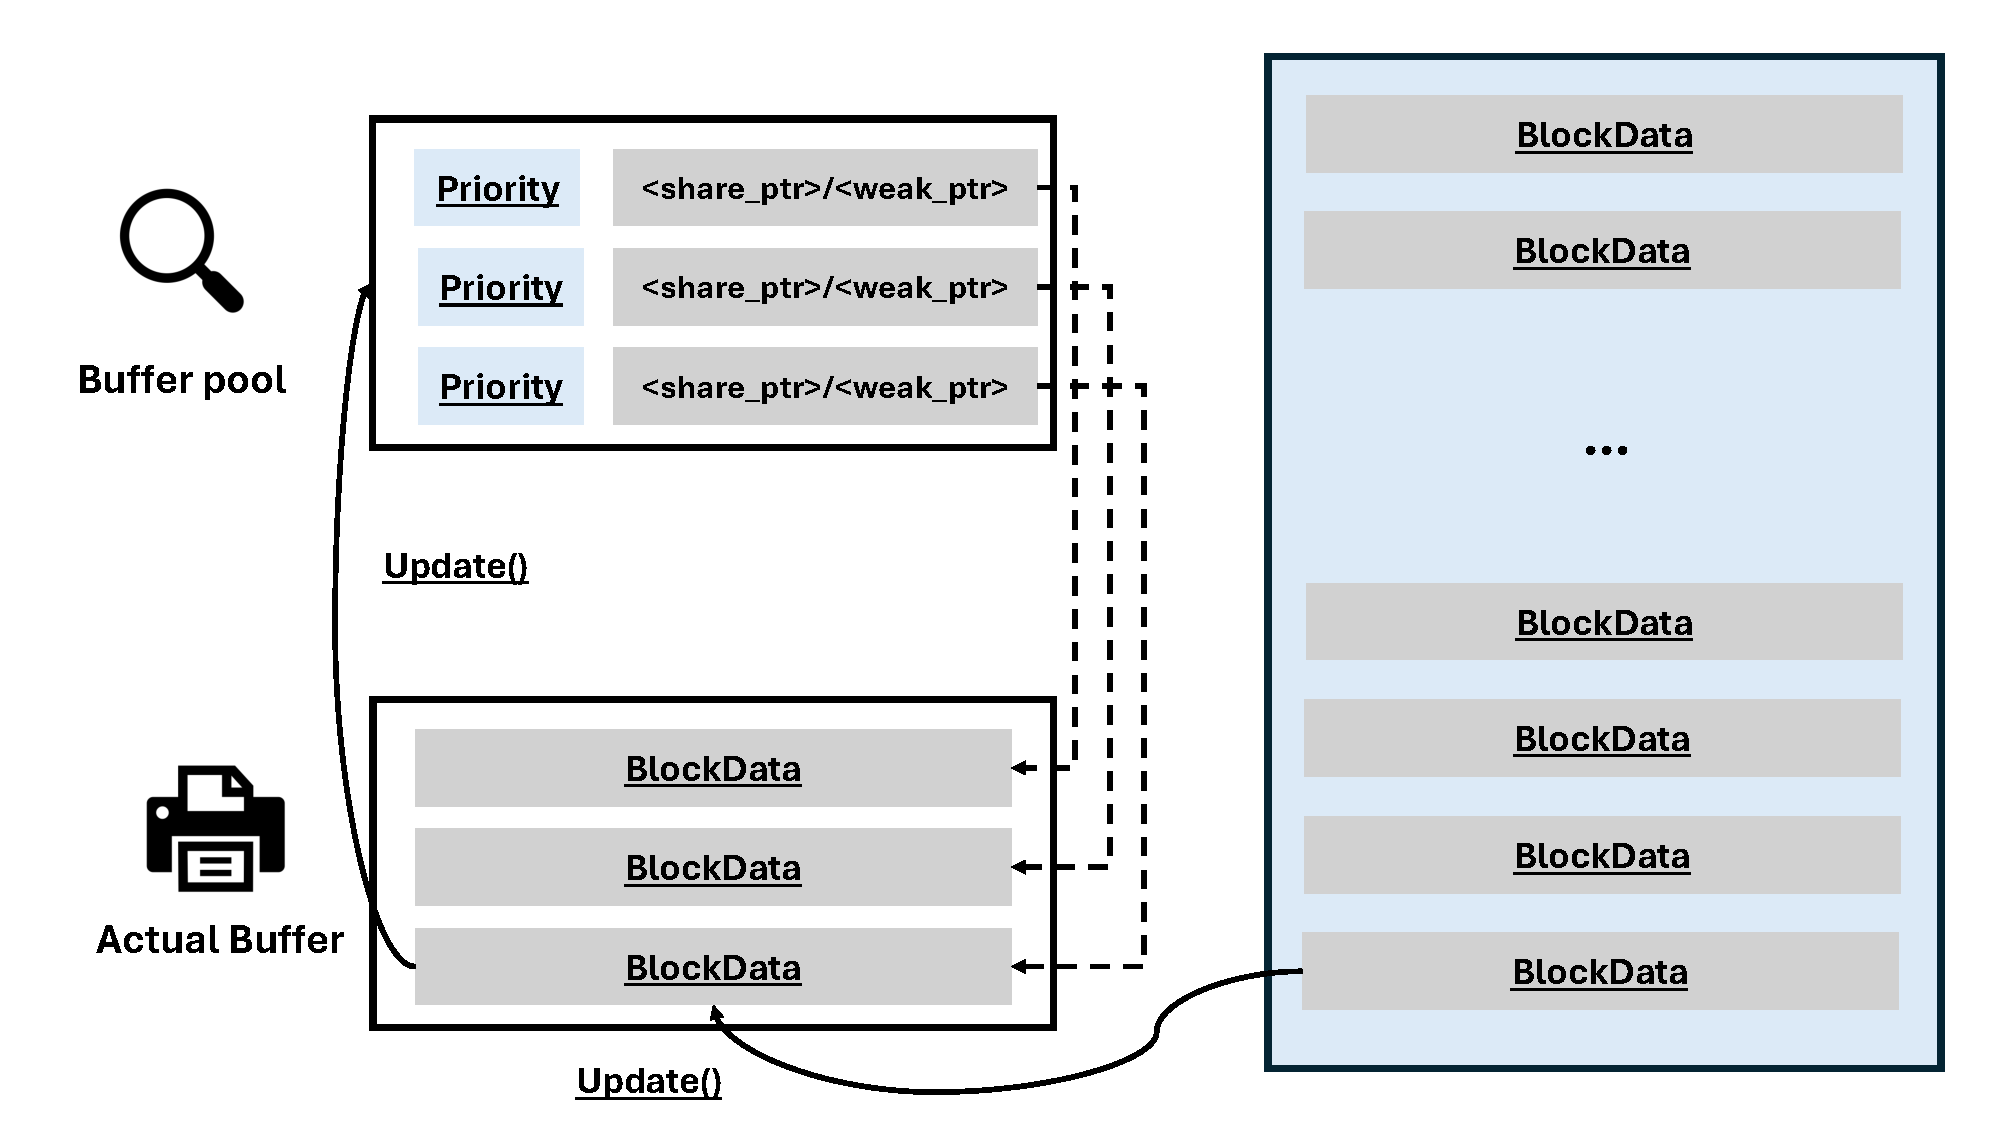
\includegraphics[width=1\linewidth]{figures/Buffer_pool.pdf}
    \caption{Design of our buffer pool. \texttt{BlockData} are shared with \texttt{shared\_ptr} or \texttt{weak\_ptr} so that no duplicate \texttt{BlockData} are constructed. During update, the data in the buffer pool will be override and the index and priority will be update}
    \label{fig:buffer-pool}
\end{figure}

We use the buffer pool to manage disk read and write operations uniformly. All database read and write operations must go through the buffer pool.

A buffer pool $\mathcal{P}$ consists of the following properties:

\begin{enumerate}
    \item A hash table $\mathcal{H}_\mathcal{P}$ in memory, using the disk offset as the key. $\mathcal{H}_\mathcal{P}(o)$ represents the block data corresponding to the disk offset $o$.

    \item A Least Recently Used (LRU) queue $\mathcal{Q}_\mathcal{P}$ that tracks the access order of frames, with the least recently used page at the head. This queue implements the page replacement policy in the buffer pool. If the page is replaced in the memory, the block data in the buffer where the old page was stored is expired; when I/O is requested to access the data block corresponding to this buffer, the data block has to be loaded from the memory to this buffer.

    \item Each frame in the buffer pool is associated with a dirty bit $\mathcal{D}$. If $\mathcal{D} = 1$, the frame has been modified in memory but not yet written back to disk. If $\mathcal{D} = 0$, the frame is synchronized with the corresponding block on disk.
\end{enumerate}

During actual I/O operations, the \texttt{FileManager} manages the buffer and reuses it if the block is already cached in the buffer pool. If the buffer pool is full, it is updated using the \textit{Least Recently Used (LRU)} policy described above. The structure of our buffer pool is illustrated in ~\Cref{fig:buffer-pool}, where each BlockData is shared using \texttt{std::shared\_ptr} or \texttt{std::weak\_ptr} to allow resource sharing. During updates, the data in the buffer is modified accordingly, and the pointers are updated to reflect the changes.

The entire structure simulates the LRU process, achieving $\mathcal{O}(1)$ time complexity for each fetch operation.


\section{Index Components}
\label{sec:index}

\subsection{B-Tree Structures}

We use a \bplustree as the implementation of the B-tree. Instead of using $n$ as a constraint, we adopted $t$ as the minimum degree of the \bplustree. So every node can have $n=2t - 1$ values and $2t$ pointers. The formal definition of our \bplustree is presented in Appendix~\ref{appendix:bplustreearch}.

In the code, we created an abstract class \texttt{BPlusTreeNode}, with the classes \texttt{BPlusTreeLeafNode} and \texttt{BPlusTreeInternalNode} inheriting from it. This abstract class can have various abstract functions such as insert, search, delete, and more. The root of the \bplustree is a \texttt{BPlusTreeNode}.

\subsection{The Bulk Loading Algorithm}

The bulk loading algorithm for constructing a \bplustree with a sorted sequence of records requires $\mathcal{O}(n)$ memory and $\mathcal{O}(n)$ disk operations, where $n$ is the number of records. If the record sequence is unsorted, an additional $\mathcal{O}(n\log n)$ memory time is needed for sorting.

We build the \bplustree layer-by-layer recursively. The \textsc{BulkLoading} function takes in a vector of pointers to records stored on disk, denoted as $\mathcal{R}$. It returns a \texttt{BPlusTreeNode} object.

\begin{algorithm}
	\caption{\textsc{BulkLoading}}
	\begin{algorithmic}
        \State $\mathcal{R} \leftarrow $ input vector
        \State $n\leftarrow$ number of records
        \State \textsc{Sort} $\mathcal{R}$ by its index
        \State $\mathcal{L} \leftarrow $ vector of \texttt{BPlusTreeLeafNode}, means the leaf layer
        \State $\ell \leftarrow\emptyset$ as the new leaf node
		\For {$r$ in $\mathcal{R}$}
        \If{$n_\ell\ge t$ and $\text{number of records remains}\ge t$}
            \State $\ell_{\mathrm{new}}\leftarrow\emptyset$ as a new leaf node
            \State $\textsc{Next}(\ell)\leftarrow\ell_{\mathrm{new}}$
            \State Append $\ell$ to $\mathcal{L}$
            \State $\ell\leftarrow\ell_{\mathrm{new}}$
        \EndIf
        \EndFor
        \State \Return \textsc{BulkLoadingUpperLayer($\mathcal{L}$)}
	\end{algorithmic} 
\end{algorithm}

Function \textsc{BulkLoadingUpperLayer} is a helper method for \textsc{BulkLoading}, which takes in a vector layer of \texttt{BPlusTreeNode}, and returns the root of the \bplustree.

\begin{algorithm}
	\caption{\textsc{BulkLoadingUpperLayer}}
	\begin{algorithmic}
        \State $\mathcal{O} \leftarrow $ input vector
        \State $n\leftarrow$ number of nodes
        \If{n = 1}
        \State\Return \textsc{First($\mathcal{L}$)}
        \EndIf
        \State $\mathcal{U} \leftarrow $ vector of \texttt{BPlusTreeInternalNode}, means the leaf layer
        \State $u \leftarrow\emptyset$ as the new internal node of the upper layer
		\For {$o$ in $\mathcal{O}$}
        \If{$n_\ell\ge t$ and $\text{number of nodes remains}\ge t$}
            \State Append $u$ to $\mathcal{U}$
            \State $u\leftarrow\emptyset$ as a new internal node of the upper layer
        \EndIf
        \EndFor
        \State \Return \textsc{BulkLoadingUpperLayer($\mathcal{U}$)}
	\end{algorithmic} 
\end{algorithm}

\subsection{Range Query on B-Tree}

\textsc{RangeQuery} is an abstract method for \texttt{BPlusTreeNode}. \textsc{RangeQuery($o, \ell, r, \mathcal{R}$)} means that the currently we are in node $o$, we want to query the records between $[\ell, r]$, and the results should be saved in $\mathcal{R}$. In real coding situations, we use dynamically to implement it. Algorithm \ref{algo:range_query} shows how the algorithm works.

\begin{algorithm}
\caption{\textsc{RangeQuery($o, \ell, r, \mathcal{R}$)}}\label{algo:range_query}
	\begin{algorithmic}
        \If{\textsc{IsLeaf($o$)}}
        \For{$i\in[0, n)$}
        \If{$k_{o}^{(i)}\ge\ell$}
        \State \textbf{continue}
        \EndIf
        \If{$k_o^{(i)}>r$}
        \State\Return
        \EndIf
        \EndFor
            \State\textsc{RangeQuery$\left(\textsc{Next($o$)}, \ell, r, \mathcal{R}\right)$}
        \Else
        \State \textsc{BinarySearch} to find the first $i$ with $k_o^{(i)}\ge \ell$
        \If {cannot find $i$}
            \State \textsc{RangeQuery$\left(s_{o}^{\left(n_s+1\right)}, \ell, r, \mathcal{R}\right)$}
        \Else
            \State \textsc{RangeQuery$\left(s_{o}^{\left(i\right)}, \ell, r, \mathcal{R}\right)$}
        \EndIf
        \EndIf
    \end{algorithmic} 
\end{algorithm}


\section{Implementation and Experiments}
\label{sec:exp}

In this section, we will show our details on our implementations and report the result as required from the 3 tasks.

\subsection{Implementation Details}
\label{subsec:implement}

This project is implemented in pure C++ using minimum version 17. The block size is determined based on the system settings and statistics of the running machine. Therefore, different machines may result in varying block sizes. For simplicity, we use a block size of 4096, which is the default setting on most machines, throughout the rest of the paper unless otherwise specified.

\subsection{Task 1}
\label{subsec:task1}

\begin{table}[ht]
    \begin{minipage}{.55\textwidth}
        \renewcommand{\arraystretch}{1.2}
        \resizebox{0.95\textwidth}{!}{
        \begin{tabular}{@{}lll@{}}
            \toprule
            \textbf{Column Name} & \textbf{Data Type} & \textbf{Row Size} (Bytes)\\
            \midrule
            \texttt{GAME\_DATE\_EST}       & \texttt{DATE}             & 10   \\
            \texttt{TEAM\_ID\_home}        & \texttt{VARCHAR(10)}      & 10  \\
            \texttt{PTS\_home}             & \texttt{INT}              &  4  \\
            \texttt{FG\_PCT\_home}         & \texttt{FLOAT32}          &  4  \\
            \texttt{FT\_PCT\_home}         & \texttt{FLOAT32}          &  4  \\
            \texttt{FG3\_PCT\_home}        & \texttt{FLOAT32}          &  4  \\
            \texttt{AST\_home}             & \texttt{INT}              &  4  \\
            \texttt{REB\_home}             & \texttt{INT}              &  4  \\
            \texttt{HOME\_TEAM\_WINS}      & \texttt{BOOLEAN}          &  1  \\
            \midrule
            \textbf{Total}        &                  & 45 \\
            \bottomrule
        \end{tabular}
        }
        \vspace{2mm}
        \caption{Fields statistics inside a record}
        \label{tab:field-stats}
    \end{minipage}
    \hfill
    \begin{minipage}{.4\textwidth}
        \centering
        \renewcommand{\arraystretch}{1.2}
        \begin{tabular}{@{}lll@{}}
        \toprule
        File                   & Num. of lines   & 26651 \\
        \midrule
        \multirow{2}{*}{Record}& Num. of records & 26651 \\
                               & Size (Bytes)    & 45    \\
        \midrule
        \multirow{2}{*}{Block} & Num. of blocks  & 293   \\
                               & Size (Bytes)    & 4096  \\
        \bottomrule
        \end{tabular}
        \vspace{5mm}
        \caption{The size of a record; The number of
records; The number of records stored in a block; The number of blocks
for storing the data}
    \end{minipage}
\end{table}

\vspace{-2mm}

\paragraph{Record} In our database system, and in the provided \textit{games.txt} file, a record consists of an array of 45 bytes. A detailed explanation of how we chose the data types and corresponding row sizes for each field is provided in \Cref{tab:field-stats}. Examples of the converted byte arrays for different data types can be found in \Cref{fig:storage-component}. Since there are 26651 lines in the txt file, there will be 26651 records in the database.

\paragraph{Block} Our block size is set to the default value of 4096 bytes. Therefore, each block can store $\left\lfloor \frac{4096}{45} \right\rfloor = 91$ records. To store all the records in our database, we will need $\left\lceil\frac{26651}{91}\right\rceil = 293$ blocks.

\paragraph{Database File} A database file in our system is a binary file named with the extension \textit{.db}. It contains multiple blocks used to store the database’s data.


\subsection{Task 2}
\label{subsec:task-2}

\paragraph{Degree $t$} In our \bplustree structure, degree (t) is the minimum number of subtrees of an internal node. In our \bplustree, the degree is $102$.

\begin{table}[h]
    \hfill
    \begin{minipage}{.99\textwidth}
        \centering
        \renewcommand{\arraystretch}{1.2}
        \begin{tabular}{@{}lll@{}}
        \toprule
        Statistic                   & Value       \\
        \midrule
        \multirow{1}{*}{Parameter \textit{n}}& 203 \\

        \midrule
        \multirow{1}{*}{Total number of nodes} & 266  \\

        \midrule
        \multirow{1}{*}{Number of levels} & 3 \\

        \midrule
        \multirow{1}{*}{Content of root node} & 3 keys from the file \\

        \bottomrule
        \end{tabular}
        \vspace{5mm}
        \caption{the parameter $n$ of the \bplustree; the
number of nodes of the \bplustree; the number of levels of the \bplustree; the content of the root node}
    \end{minipage}
\end{table}

\paragraph{Parameter $n$} The parameter $n$ is restricted to be an odd integer, which refers to the maximum number of keys that can be stored in a node; and it is equal to two times degree minus $1$, which is $2\times 102-1=203$.

\paragraph{Number of Nodes} There are $26,651$ records. Since each leaf node must store at least $102$ keys, the minimum number of leaf nodes is $\left\lceil\frac{26651}{102}\right\rceil = 262$, So there will be $262$ leaf nodes in this case. Each internal node can have at least $102$ pointers (since internal nodes must have at least
$t=102$ children). Therefore, the number of internal nodes at the first level is $\left\lceil \frac{262}{102} \right\rceil = 3$. Since there are only $3$ internal nodes in the first level, the second level will contain $1$ root node (because the root can store at least $101$ keys and have up to $102$ children). Therefore, totally there are $262 + 3 + 1 = 266$ nodes.

\paragraph{Number of levels in the \bplustree} For leaf level there are 262 leaf nodes; at first internal level there are 3 internal nodes; at root Level there are 1 root node. Therefore, the \bplustree has \textbf{3 levels}.

\paragraph{Content of the root node (only the keys)} The root node will contain the first keys from each of its 3 children (the internal nodes). Since there are only 3 internal nodes, the root will contain 3 keys that guide the search process to the appropriate internal node.

\subsection{Task 3}
\label{subsec:task-3}

\begin{figure*}[h]
    \centering
    \begin{subfigure}[t]{0.45\textwidth}
        \centering
        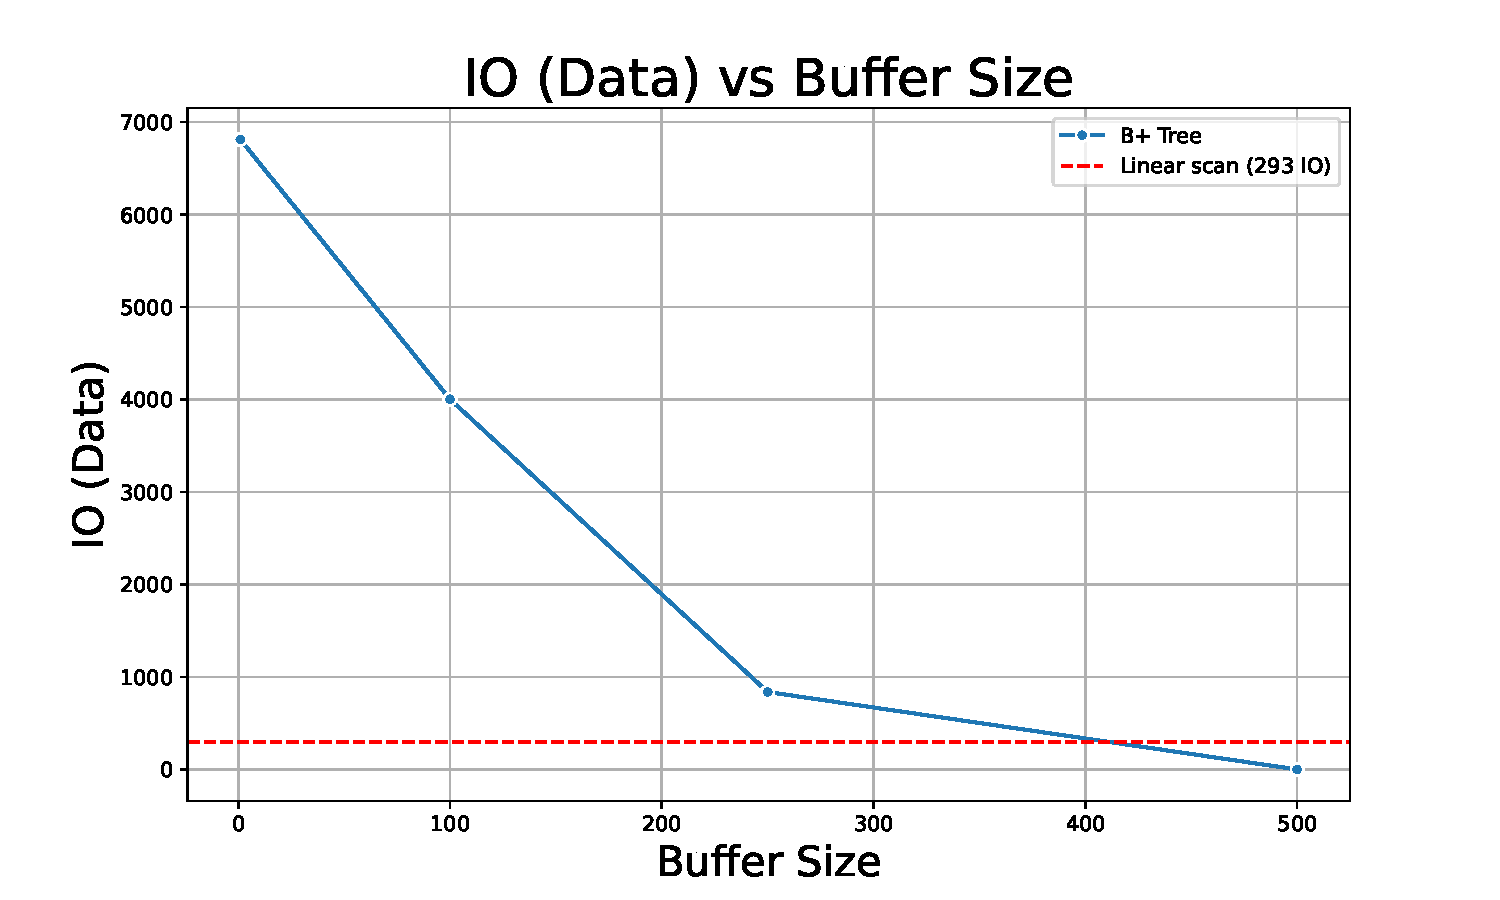
\includegraphics[width=0.95\linewidth]{figures/block_io_vs_buffer_size.pdf}
        \caption{Comparison between different buffer size and data block access for \bplustree}
    \end{subfigure}%
    ~
    \begin{subfigure}[t]{0.45\textwidth}
        \centering
        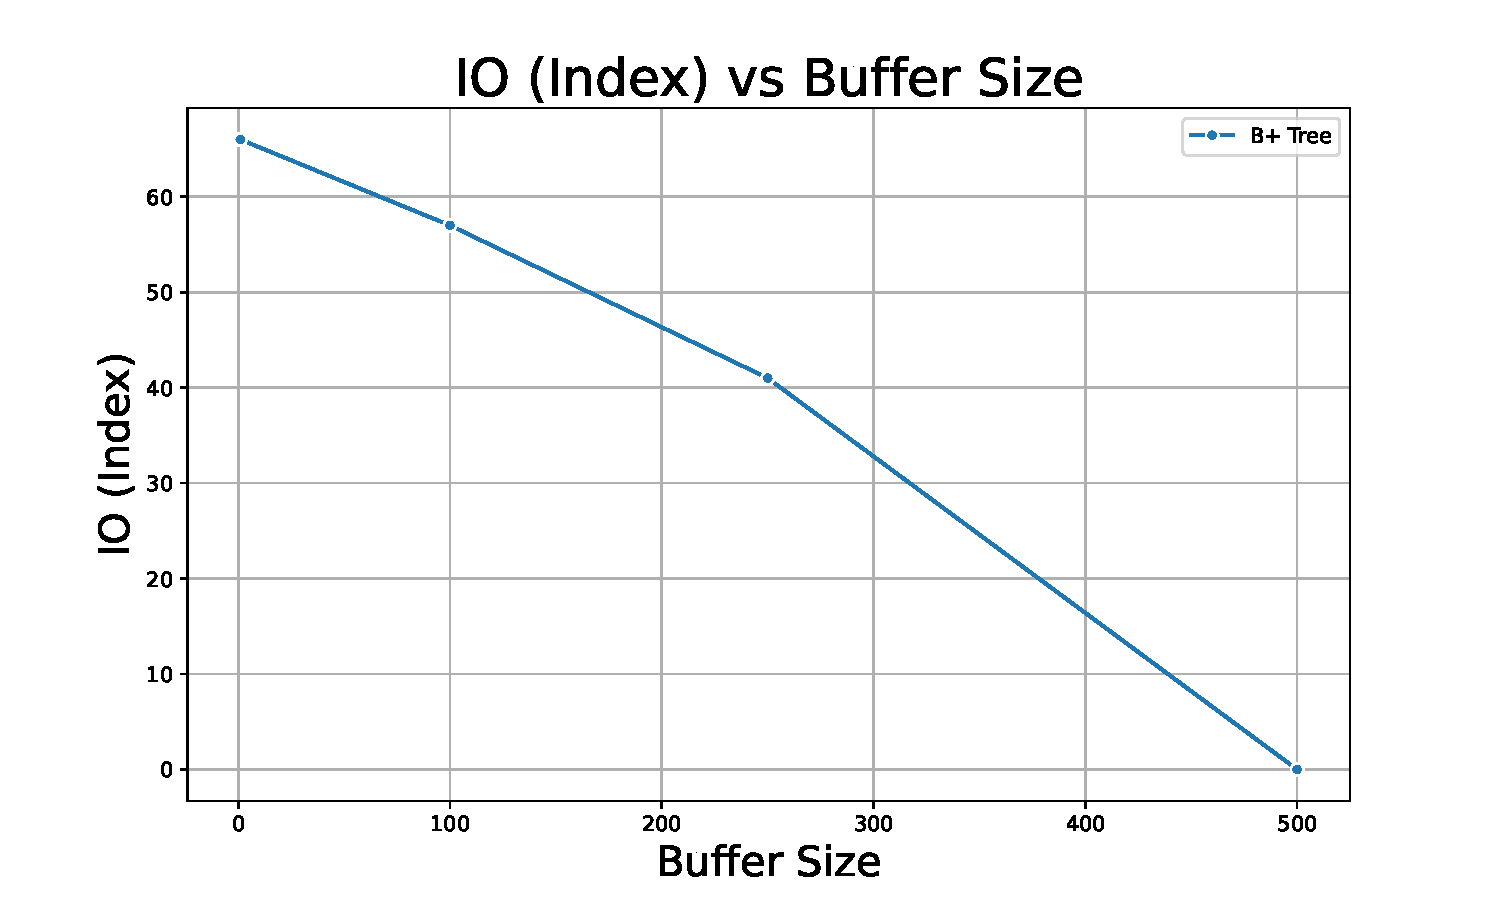
\includegraphics[width=0.95\linewidth]{figures/index_io_vs_buffer_size.pdf}
        \caption{Comparison between different buffer size and index block access for \bplustree}
    \end{subfigure}
    \vspace{3mm}

    \begin{subfigure}[t]{0.55\textwidth}
        \centering
        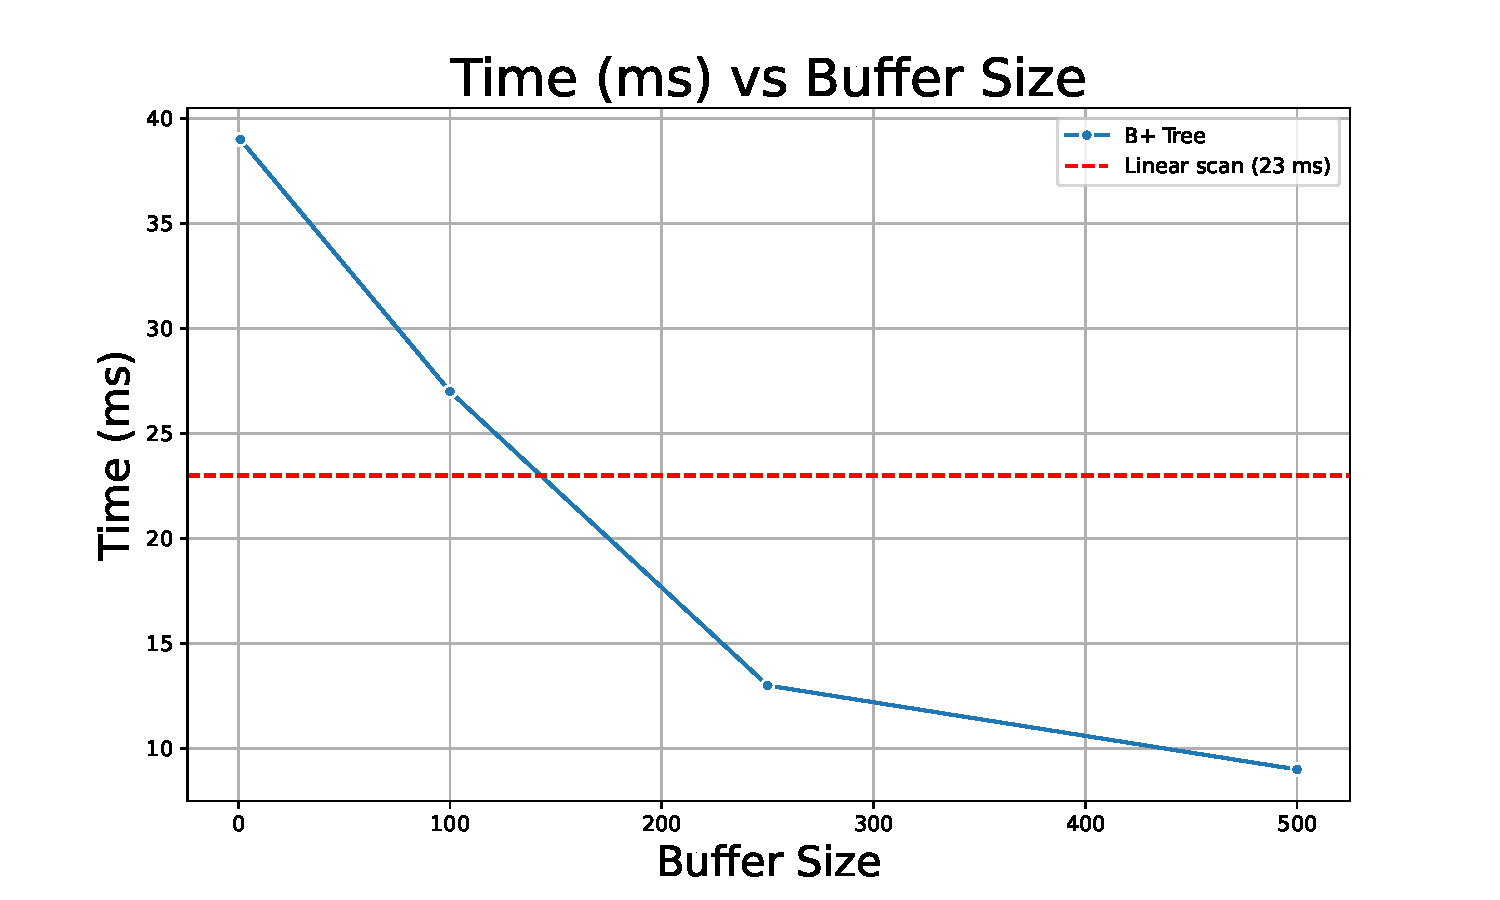
\includegraphics[width=0.95\linewidth]{figures/time_vs_buffer_size.pdf}
        \caption{Comparison between different buffer size and runtime for \bplustree and linear scan}
        \label{subfig:time-vs-buffer}
    \end{subfigure}
    \caption{Exploring different buffer size}
\end{figure*}


\begin{table}[h]
\begin{minipage}{0.55\textwidth}
\resizebox{0.95\textwidth}{!}{
\begin{tabular}{@{}l|ll|ll}
\toprule
Buffer Size & \textsc{Time} ($\mu s$) & \textsc{Time} ($ms$) & \textsc{IO} (Index Block) & \textsc{IO} (Data Block)  \\
\midrule
1            & 39774              & 39       & 66   &   6812 \\
% 10           & 39810              & 39       & 87   &   6265 \\
% 50           & 34176              & 34       & 114  &   5100 \\
100          & 27891              & 27       & 57   &   4003 \\
250          & 13469              & 13       & 41   &   838  \\
500          & 9351               & 9        & 0    &   0    \\
\bottomrule
\end{tabular}
}
\vspace{2mm}
\caption{The number of IO and time for different buffer sizes using B+ tree. Our indexes are built in a non-clustered order and thus may access a data block multiple times and getting the result}
\label{tab:io-tab}
\end{minipage}
\hfill
\begin{minipage}{0.4\textwidth}

\resizebox{0.95\textwidth}{!}{
\centering
\renewcommand{\arraystretch}{1.2}
\begin{tabular}{l|ccc}
\toprule
Method           & IO (Index) & IO (Data) & Time (ms) \\
\midrule
Linear Scan      & 0          & 293       & 22        \\
\bplustree          & 66         & 6812      & 39        \\
\bplustree w. cache & 41         & 838       & 13        \\
\bottomrule
\end{tabular}
}
\vspace{2mm}
\caption{Comparison with different methods: Linear Scan, B+ tree, B+ tree with cache. The cache of the B+ tree is set to be 250 pages.}
\label{tab:comparison}

\end{minipage}

\end{table}

We will now present the statistics required for Task 3. The results were obtained by running the system with different buffer sizes, and the outcomes are summarized in \Cref{tab:io-tab,tab:comparison}.

\paragraph{Index Node Access} Without using a buffer\footnote{The minimum buffer size for our program is 1 since we always update our buffer after reading one block. However, in this scenario, this buffer would not have any effect. Thus, we consider the case when buffer size is 1 as no buffer.}, the number of I/O operations for accessing index blocks is 66, which is approximately equal to $\lfloor \frac{6902}{102} \rfloor = 67$, where 6902 is the number of records that satisfy the query conditions. As the buffer size increases, the number of I/O operations for accessing the index decreases gradually, as portions of the index are stored in the buffer during the building phase.

\paragraph{Data Block Access} Since we use a dense non-clustered index, many data blocks are accessed multiple times because the records are not stored sequentially, the number of I/O operations for accessing data blocks is 6812, which is much greater than using linear scan. The high I/O in data block access results in the runtime of the B+ tree being longer than that of the range query. This issue can be mitigated by increasing the buffer size, as the linear scan cannot fully utilize the buffer, and the B+ tree will have a shorter runtime with an increased buffer size.

\paragraph{Average of ``\texttt{FG3\_PCT\_home}'' for the Records} The average ``\texttt{FG3\_PCT\_home}'' value retrieved from the returned records is 0.420801. We verified this result using a simple \texttt{Python} program, which returned a value of 0.4208015. Thus, we confirm that the query result is accurate.

\paragraph{Running Time} The algorithm's running time without using a buffer is approximately 39 ms. As the buffer size increases, the running time decreases to around 9 ms. Detailed statistics can be found in \Cref{tab:io-tab}.

\paragraph{Data Blocks Accessed by Linear Scan} The number of data blocks accessed by a brute-force linear scan is constant at $\left\lceil \frac{26651}{102} \right\rceil = 293$.

\paragraph{Running Time of Linear Scan} The running time for the linear scan is constant, taking approximately 22 ms. A detail comparison can be found in \Cref{subfig:time-vs-buffer}


\section{Conclusion}
In this report, we present our design of our storage and index components for the database system in \Cref{sec:storage,sec:index}. We then report all of our statistics and experiment results in \Cref{sec:exp} that is required from the manual.


\bibliographystyle{plain} % or another style like apalike, abbrvnat, etc.
\bibliography{references/ref} % assumes you have a references.bib file

\newpage
\appendix

\section{Formal Definition of Our B Plus Tree}
\label{appendix:bplustreearch}

Our \bplustree is constructed following the foundational definition of B-trees as given in \cite{cormen2022introduction}, with key modifications to accommodate the structure and search needs of our data storage and indexing system.

The primary difference between our \bplustree and the one in \cite{cormen2022introduction} is that in our implementation is that only the leaf nodes store the actual data records, while internal nodes store only the keys.

\subsection{Node Structure}

Each node $x$ in the \bplustree has the following properties:\begin{enumerate}
        \item \textbf{Number of Keys:} $n_x$, representing the number of keys currently stored in node $x$. For internal nodes, these keys help guide the search by partitioning the search space.
        \item \textbf{Keys:} The $n_x$ keys, $k^{(1)}_x,k^{(2)}_x,\cdots,k^{(n_x)}_x$, stored in monotonically increasing order, such that $k^{(1)}_x<k^{(2)}_x<\cdots<k^{(n_x)}_x$,
        \item \textbf{Leaf Indicator:} $\ell_x$, a boolean value that is \texttt{true} if $x$ is a leaf and \texttt{false} if $x$ is an internal node.
        \item \textbf{Pointers:} Each node, depending on weather it is an internal or leaf node, contains a specific number of pointers (described in the next sections) that link to either child nodes or data blocks
    \end{enumerate}

\subsection{Internal Nodes}

Each internal node $x$ contains $n_x + 1$ pointers, denoted  $s^{(1)}_x,s^{(2)}_x,\cdots,s^{(n_x + 1)}_x$, which point to its child nodes. These pointers separate the key space such that each pointer directs the search towards the subtree containing the relevant keys.
        \begin{itemize}
            \item \textbf{Pointers as Navigational Aids}: The internal nodes do not store actual data records but only serve as guides for navigating to the correct leaf node or subtree where the data is stored.
        \end{itemize}
        \begin{itemize}
            \item \textbf{Key-based Navigation}: The keys in an internal node are used to define search boundaries. If a search for a key \textit{k} lands in node \textit{x}, then the key is passed to the appropriate child pointer based on the relationship: $$k_1<k_x^{(1)}\le k_2<k_x^{(2)}\le \cdots <k_x^{(n_x)}\le k_{n_x+1}$$
where $s^{(i)}_x$ leads to the subtree containing all keys in the range defined by the keys in the parent node.
        \end{itemize}

\subsection{Leaf Nodes}

Each leaf node $x$ contains $n_x + 1$ pointers, denoted $s^{(1)}_x,s^{(2)}_x,\cdots,s^{(n_x + 1)}_x$, which are structured differently from the internal node pointers:

        \begin{enumerate}
            \item For $1\le i\le n_x$,each pointer $s^{(i)}_x$ points directly to the data record corresponding to the key $k_x^{(i)}$.
            \item The last pointer, $s^{(n_x+1)}_x$ points to the \textbf{next leaf node} in the \bplustree's depth-first search (DFS) order. This allows for efficient range queries by following the chain of leaf nodes:\begin{itemize}
            \item If $x$ is the last leaf node, then $s^{(n_x+1)}$ is $\emptyset$, indicating the end of the tree.\end{itemize}
        \end{enumerate}


\subsection{Key Separation in Subtrees}

The keys $k_x^{(i)}$ separate the ranges of keys stored in each subtree. For any key subtree, $k_i$ is stored in the subtree with root $s_x^{(i)}$, the following relationship holds:  $$k_1<k_x^{(1)}\le k_2<k_x^{(2)}\le \cdots <k_x^{(n_x)}\le k_{n_x+1}$$

This property ensures that a search operation is guided down the correct subtree by comparing the key against the keys in the parent node.

\subsection{Leaf Depth}
All leaf nodes in the \bplustree are located at the same depth, equal to the height $h_T$ of the tree. This ensures balanced access times for all records, as every search or insertion operation requires traversing the same number of levels to reach a leaf node.

\subsection{Key Boundaries and Node Capacity}
Each node in the \bplustree has lower and upper bounds on the number of keys it can hold, based on the integer parameter $t\ge 2$:
\begin{enumerate}
    \item Lower Bound:
    \begin{itemize}
        \item Any node(except the root) must contain at least $t-1$ keys.
        \item Each internal node, therefore, has at least $t$ children.
        \item The root node may contain fewer than $t-1$ keys but must contain at least one key if the tree is non-empty.
    \end{itemize}

    \item Upper Bound:
    \begin{itemize}
        \item Any node can hold a maximum of $2t-1$.
        \item An internal node can have up to $2t$ children, allowing for balanced growth as new records are inserted.
    \end{itemize}

\end{enumerate}

\subsection{Operations on the B+ Tree}

\begin{itemize}
    \item \textbf{Search:} To locate a record, the search process navigates from the root to the appropriate leaf node, using the keys in internal nodes to direct the search path. Once the correct leaf node is located, the corresponding data is fetched via the leaf node’s pointers.
    \item \textbf{Insertion:} Insertion occurs by first finding the correct leaf node for the key. If the leaf node has space for additional keys, the new key and data record are added. If the leaf is full, it is split, and a new key is promoted to the parent node. If the parent node also becomes full, the splitting and promotion process continues recursively, potentially resulting in the tree growing in height.
    \item \textbf{Range Queries:} Range queries are highly efficient in the \bplustree due to the linked list structure of the leaf nodes. Once the range's starting key is located, the query can traverse the linked list of leaf nodes to retrieve all records within the specified range.
\end{itemize}


\end{document}